\documentclass[11pt,a4paper]{article}

\usepackage[utf8]{inputenc}
\usepackage[T1]{fontenc}
\usepackage[portuguese]{babel}
\usepackage{lmodern}
\usepackage[margin=2.2cm]{geometry}
\usepackage{graphicx}
\usepackage{booktabs}
\usepackage{xcolor}
\usepackage{float}
\usepackage{caption}
\usepackage{enumitem}
\usepackage[hidelinks]{hyperref}

\definecolor{azul}{HTML}{3A6EA5}
\definecolor{fundo}{HTML}{F3F6FA}

% legendas das capturas: "Captura N" (evita confusão com os números das figuras do projeto)
\addto\captionsportuguese{\renewcommand{\figurename}{Captura}}

\setlist{itemsep=2pt, topsep=4pt}
\setlength{\parindent}{0pt}
\setlength{\parskip}{5pt}

% Campos de cada alteração: data, ficheiros, figuras, commit, autoria
\newcommand{\ficha}[5]{%
  \begin{center}
  \colorbox{fundo}{\begin{minipage}{0.95\linewidth}\small
  \begin{tabular}{@{}p{3.2cm}p{11.8cm}@{}}
  \textbf{Data} & #1\\
  \textbf{Ficheiros} & #2\\
  \textbf{Figuras afetadas} & #3\\
  \textbf{Commit} & #4\\
  \textbf{Autoria} & #5\\
  \end{tabular}
  \end{minipage}}
  \end{center}}

\title{\color{azul}\textbf{Registo de alterações}\\[4pt]
\large Visualização de Dados 2026/27 --- Projeto NYPD, Grupo E}
\date{}

\begin{document}
\maketitle

Este documento regista as alterações feitas ao projeto a partir de 27 de novembro de 2026,
com a justificação de cada uma e o antes e depois das figuras afetadas. Serve de apoio ao
artigo final (PD) e à discussão na apresentação, onde é pedido que o grupo explique porque
mudou uma figura ou descartou uma opção.

\tableofcontents

% ==============================================================================
\section*{Ponto de partida}
\addcontentsline{toc}{section}{Ponto de partida}

Estado do projeto no commit \texttt{fdb1535} (27 nov 2026), antes das alterações registadas abaixo:

\begin{itemize}
  \item Análise de crime de rua em \texttt{R/trabalho\_vd.ipynb}, com 8 figuras em \texttt{fig/}.
  \item O notebook corre no computador (VS Code, kernel R) e no Colab sem alterações:
        lê os dados de \texttt{data/} e grava as figuras em \texttt{fig/} a 300 dpi.
  \item Hipótese testada: \emph{os homens são a maioria das vítimas em todas as infrações de rua}
        (rejeitada: são a maioria em 7 das 8 infrações principais, mas não em \textit{Harassment 2}).
\end{itemize}

% ==============================================================================
\section{Figura 2: escolher as 8 infrações pelas queixas com vítima pessoa}

\ficha{27 nov 2026}
      {\texttt{R/trabalho\_vd.ipynb} (cálculo de \texttt{top8})}
      {\texttt{fig/figura\_rua\_2\_infracoes.png}}
      {o commit que acrescenta esta entrada (\texttt{git log -{}- alteracoes/})}
      {Matilde (27 nov, 14:07: \texttt{fm} no lugar de \texttt{st\_base})}

\subsection*{O que mudou}

As 8 infrações da Figura 2 eram escolhidas pelo número total de queixas de rua
(\texttt{st\_base}). Passam a ser escolhidas pelo número de queixas \textbf{com vítima homem ou mulher}
(\texttt{fm}), que é a mesma base usada para calcular as percentagens do gráfico.

\begin{center}\small
\begin{tabular}{@{}ll@{}}
\toprule
\textbf{Antes} & \textbf{Depois}\\
\midrule
\texttt{top8 <- st\_base \%>\%} & \texttt{top8 <- fm \%>\%}\\
\bottomrule
\end{tabular}
\end{center}

\subsection*{Justificação}

A Figura 2 mostra a percentagem de \emph{vítimas} homens e mulheres. Uma infração só faz sentido
no gráfico se tiver vítimas que são pessoas. Com o critério antigo, duas infrações entravam no
top 8 por terem muitas queixas, mas quase sem vítimas pessoa:

\begin{center}\small
\begin{tabular}{@{}lrrr@{}}
\toprule
\textbf{Infração} & \textbf{Queixas de rua} & \textbf{Com vítima pessoa} & \textbf{\%}\\
\midrule
DANGEROUS DRUGS          & 43\,863 & 427     & 1\,\%\\
VEHICLE AND TRAFFIC LAWS & 88\,275 & 33\,274 & 38\,\%\\
\bottomrule
\end{tabular}
\end{center}

\begin{itemize}
  \item Em \textbf{Dangerous Drugs}, a vítima é o Estado de Nova Iorque (\texttt{vic\_sex = E})
        em 43\,315 queixas. Segundo o dicionário de dados, \texttt{E} não é uma pessoa. A barra
        mostrava 68\,\% de homens calculados sobre apenas 427 queixas (1\,\% da infração), o que
        dava ao leitor uma ideia errada da importância dessa barra.
  \item \textbf{Vehicle and Traffic Laws} tem o mesmo problema em menor grau: 62\,\% das queixas
        não têm uma pessoa como vítima.
  \item Contar o top 8 na mesma base das percentagens (\texttt{fm}) torna o critério coerente:
        \emph{as 8 infrações de rua com mais vítimas homens ou mulheres}.
\end{itemize}

\textbf{Alternativa considerada e descartada:} retirar só Dangerous Drugs e manter o critério
antigo (entraria Felony Assault). Foi descartada porque deixava Vehicle and Traffic Laws no
gráfico com o mesmo problema.

\subsection*{Efeito no gráfico e nas conclusões}

\begin{itemize}
  \item \textbf{Saem:} Dangerous Drugs e Vehicle and Traffic Laws.
  \item \textbf{Entram:} Robbery (77\,\% homens, $n = 40\,905$) e Felony Assault (75\,\% homens, $n = 38\,218$).
  \item As outras 6 infrações mantêm-se com os mesmos valores.
  \item \textbf{A conclusão da hipótese não muda:} os homens continuam a ser a maioria das vítimas
        em 7 das 8 infrações e \textit{Harassment 2} continua a ser a exceção (55\,\% mulheres).
\end{itemize}

\begin{figure}[H]
  \centering
  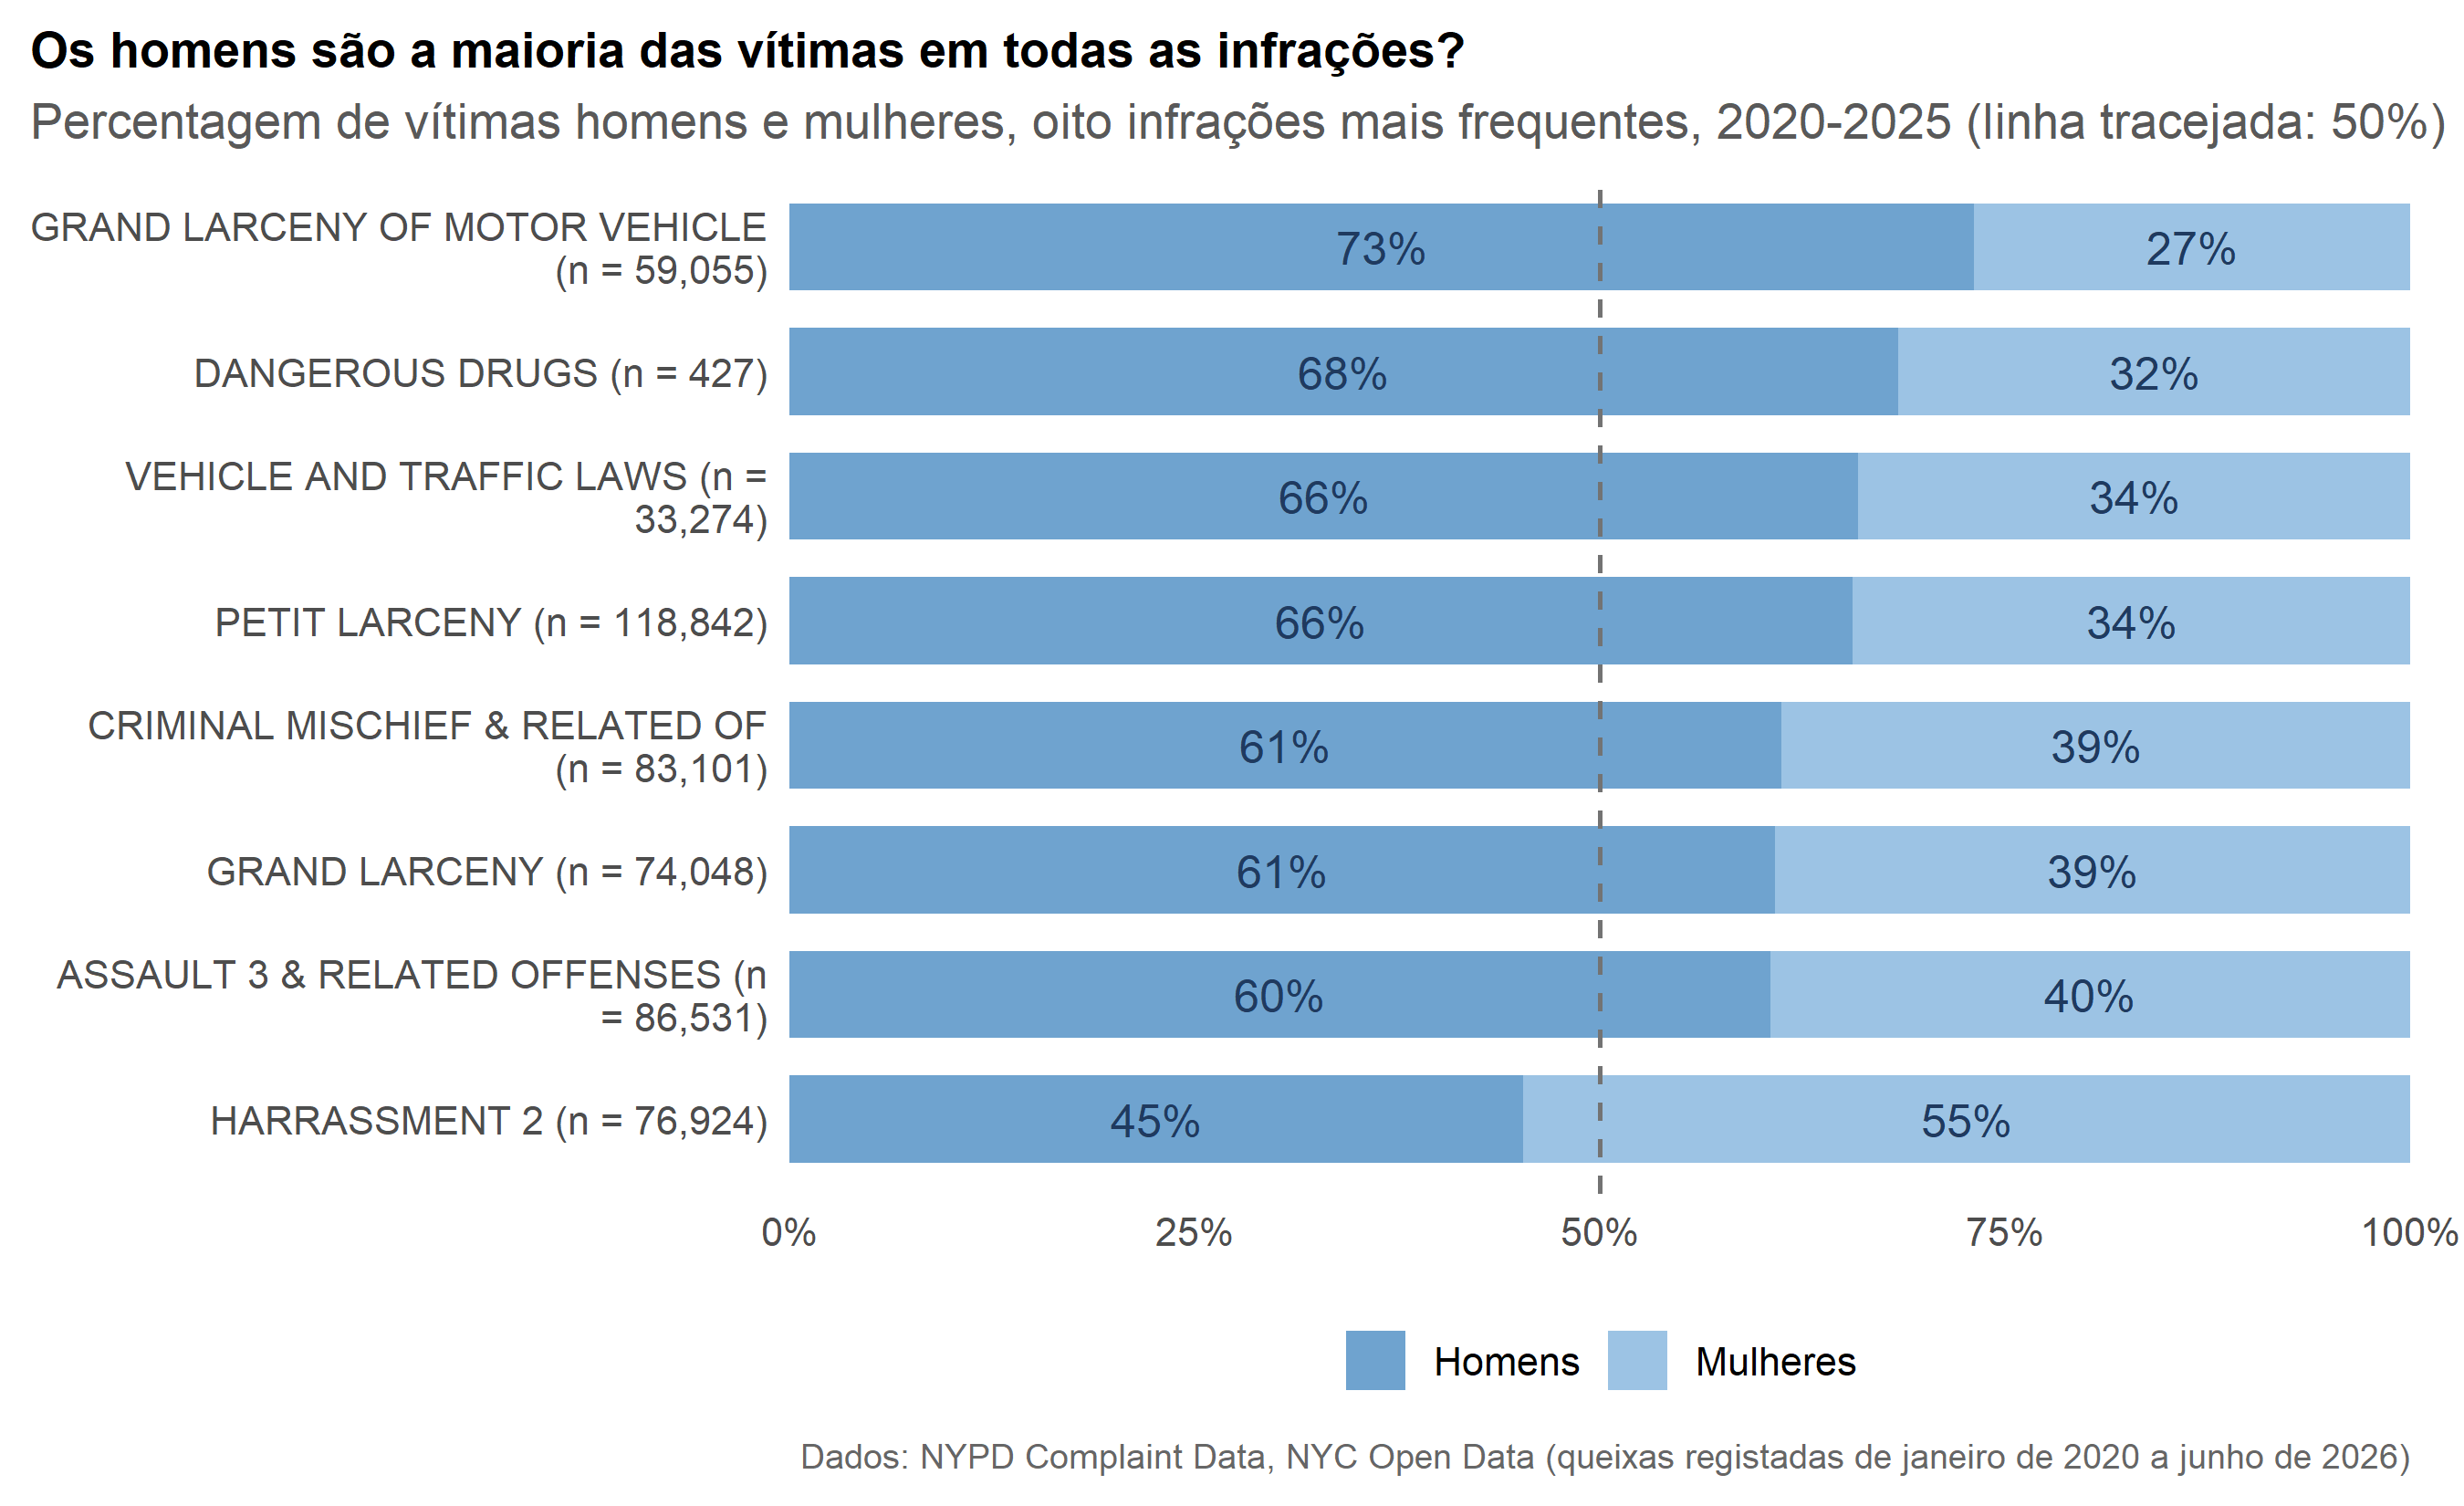
\includegraphics[width=0.85\linewidth]{img/01_fig2_antes.png}
  \caption{Figura 2 \textbf{antes}: inclui Dangerous Drugs ($n = 427$) e Vehicle and Traffic Laws.}
\end{figure}

\begin{figure}[H]
  \centering
  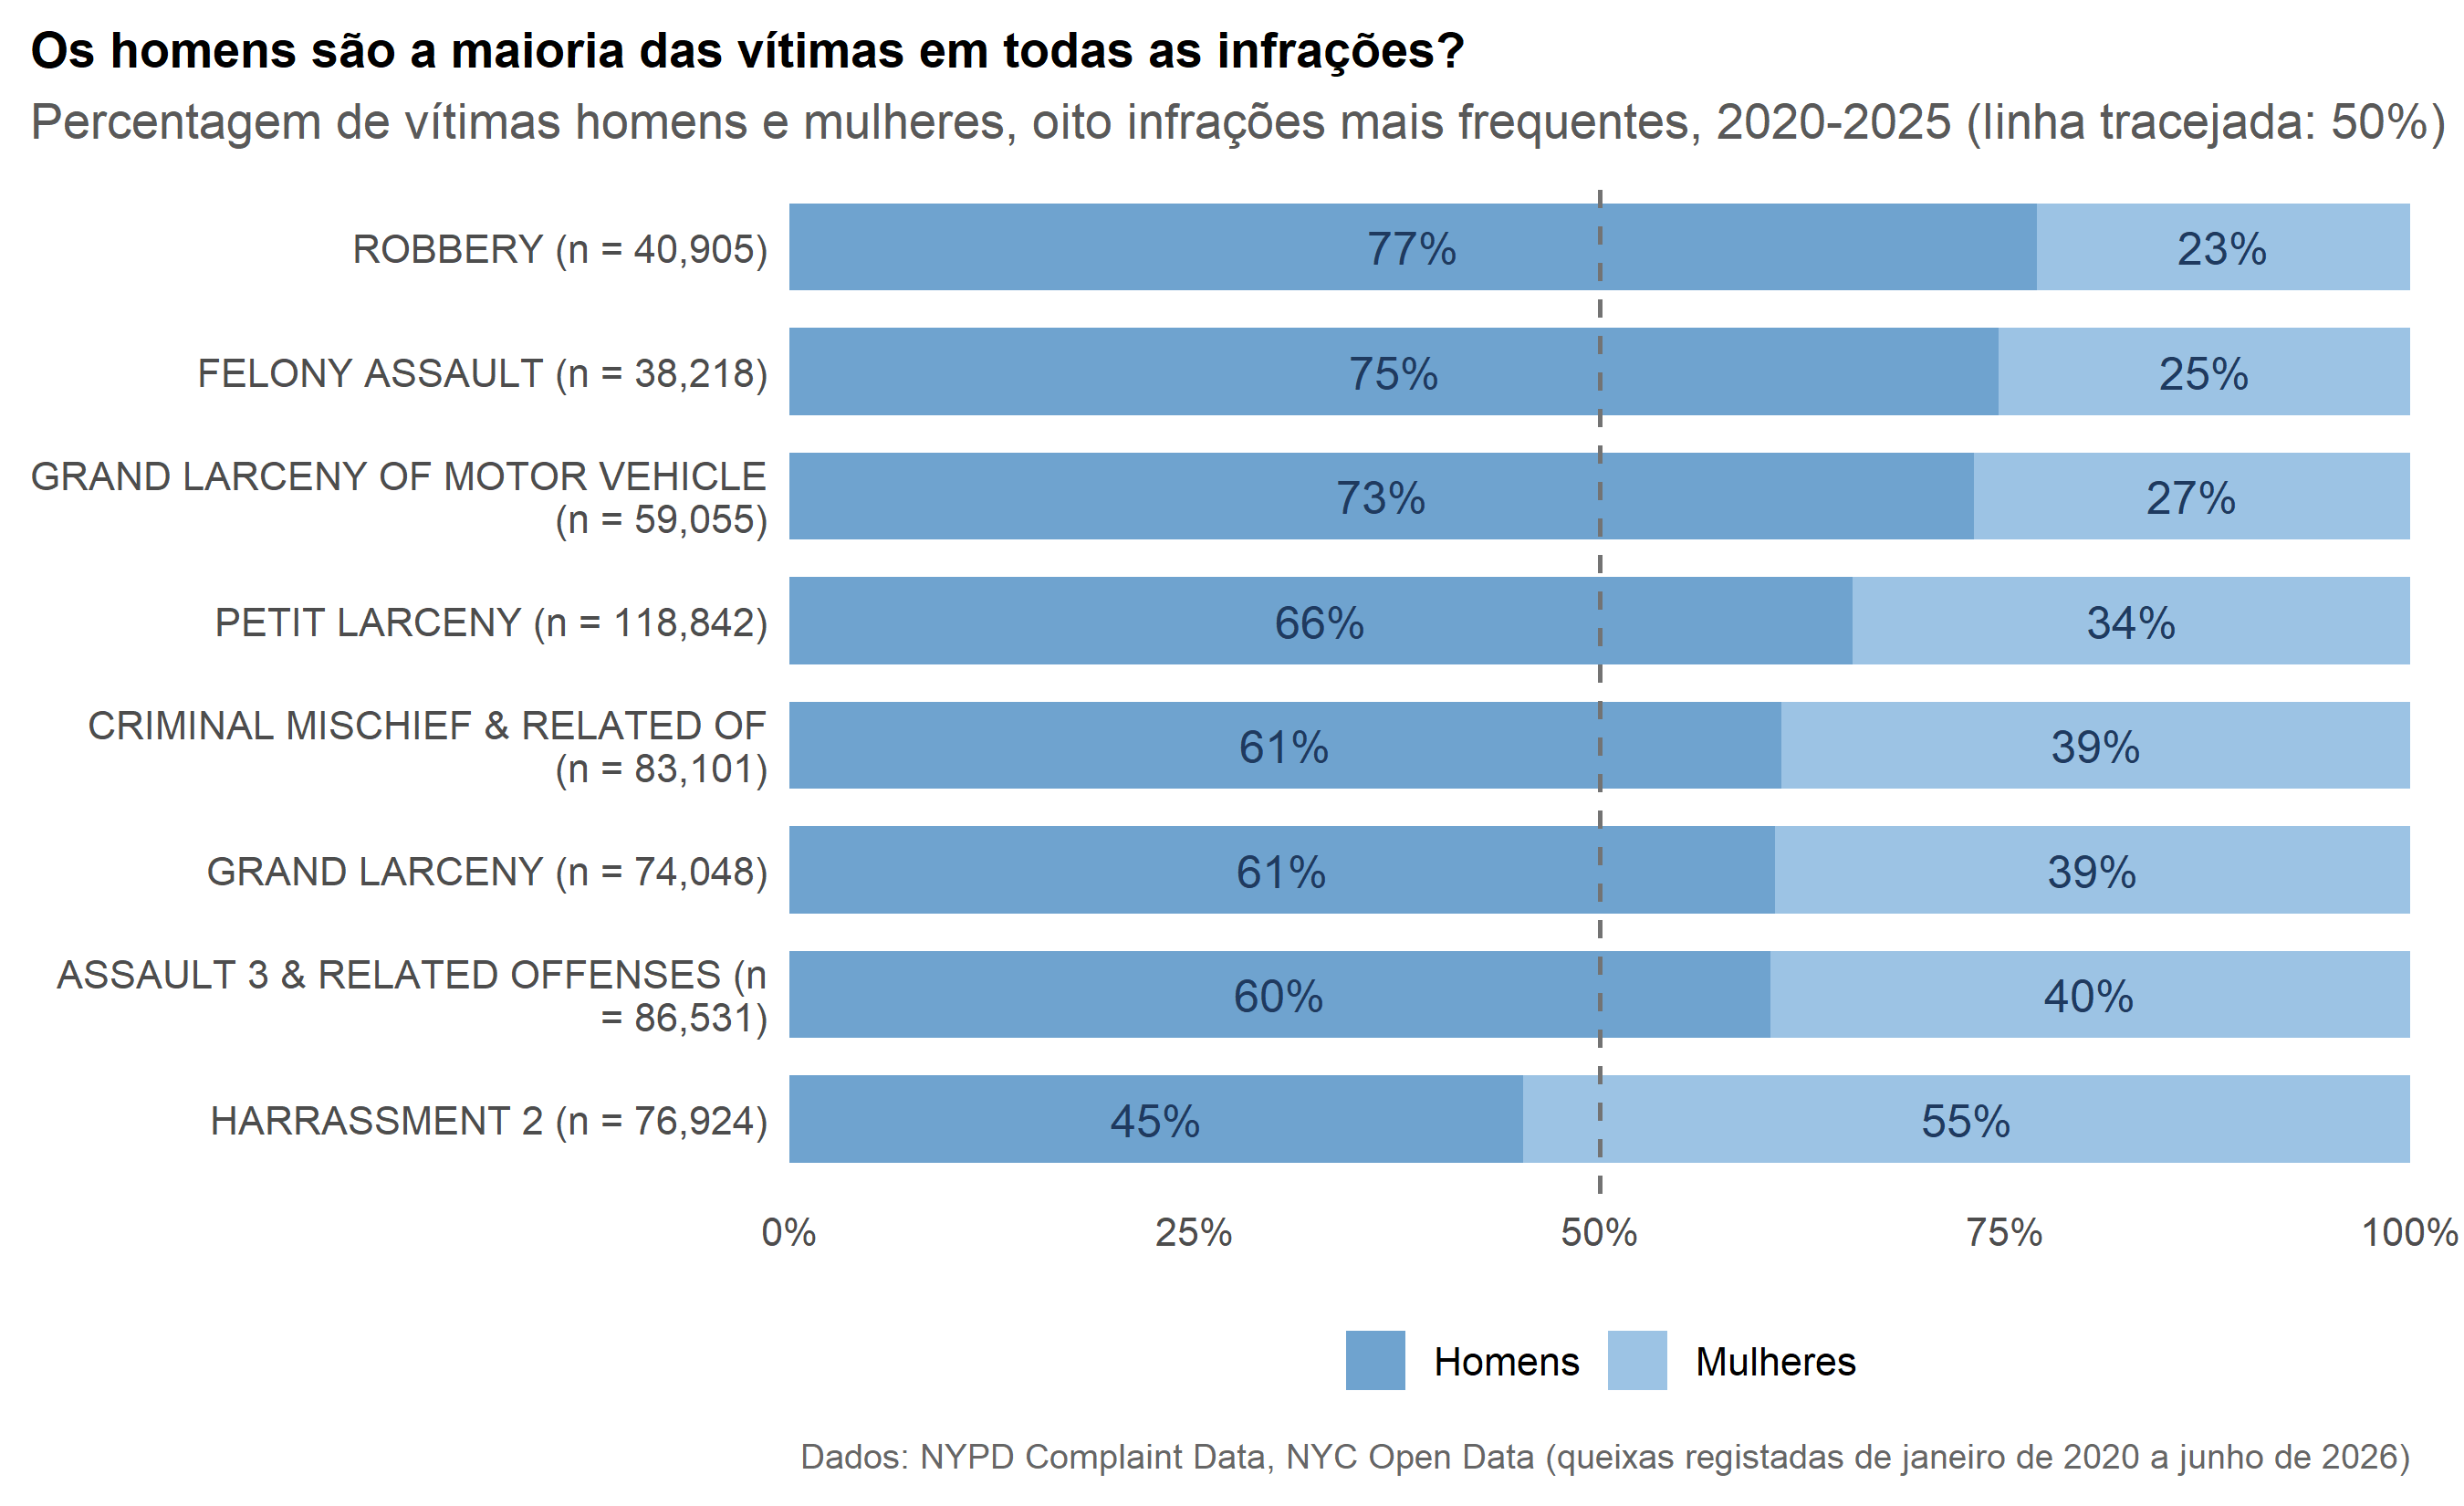
\includegraphics[width=0.85\linewidth]{img/01_fig2_depois.png}
  \caption{Figura 2 \textbf{depois}: as 8 infrações com mais vítimas homens ou mulheres.}
\end{figure}

% ==============================================================================
% MODELO PARA NOVAS ALTERAÇÕES (copiar, numerar e preencher)
%
% \section{Título curto da alteração}
% \ficha{data}{ficheiros alterados}{figuras afetadas}{commit}{autoria}
% \subsection*{O que mudou}
% \subsection*{Justificação}
% \subsection*{Efeito no gráfico e nas conclusões}
% figuras antes/depois em img/NN_nome_antes.png e img/NN_nome_depois.png
% ==============================================================================

\end{document}
